\documentclass{article}
\usepackage[utf8]{inputenc}

\title{Raport - Congressional voting}
\author{Yevhenii Vinichenko, Krzysztof Wolny}
\date{April 2021}

\usepackage{natbib}
\usepackage{graphicx}

\begin{document}

\maketitle

\section{Opis problemu}

Naszym celem było stworzenie modelu predykcyjnego, który przewidywałby na podstawie głosów kongresmana z Izby Reprezentantów Stanów Zjednoczonych, czy jest on demokratem, czy republikanem. 

\section{Opis zbioru danych}

Otrzymaliśmy zbiór danych o głosach kongresmenów z Izby Reprezentantów Stanów Zjednoczonych. W danych były zapisane wyniki, czy dany kongresmen głosował za, przeciw, czy wstrzymał się od głosu w danej propozycji. Łącznie propozycji było 16. W dataframie litera 'y' oznaczała poparcie kongresmana dla tej propozycji, 'n' głos przeciwko, a '?' wstrzymanie się od głosu. W danych była również informacja, czy kongresman jest demokratem, czy republikanem.

Dane, które otrzymaliśmy, tak jak wynika z opisu, były dyskretne. Po przeanalizowaniu danych udało nam się znaleźć kilka propozycji, które w wyraźny sposób odróżniały republikanów od demokratów. Jest to oczywiście bardzo dobra informacja w kontekście tworzenia modeli.

\begin{figure}
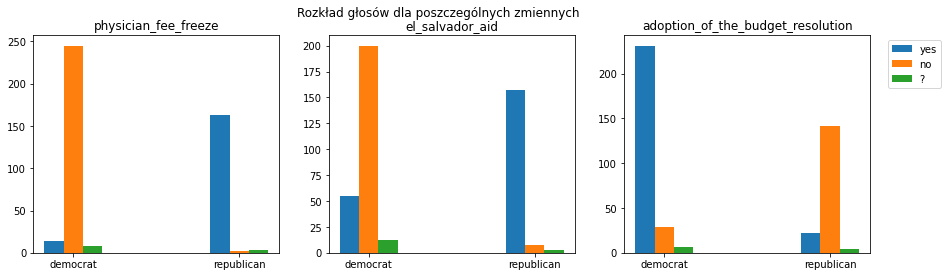
\includegraphics[width=15cm]{zdjecia/wykres.png}
\end{figure}

\section{Preproccessing}

Z związku z tym, że nasze dane były dyskretne nie potrzebowaliśmy robić dużej ilości preproccessingu. Naszym głównym celem było zamienienie oznaczeń literowych na liczbowe, aby ułatwić obliczenia. Postanowiliśmy zamienić dane w następujący sposób: 

\subsection{Wcześniejsze błędy}

W kamieniu milowym numer 2 traktowaliśmy '?' jako NaN i próbowaliśmy uzupełniać te dane. Nie jest to jednak najlepsze myślenie, ponieważ wstrzymanie się od głosów również jest częścią polityki. Były nawet takie propozycje, w których większość polityków wstrzymywało się od głosu. Modele statystyczne, które stworzyliśmy pracują również z większą skutecznością, gdy uznajemy '?' jako oddzielną zmienną. 

\section{Modele statystyczne}

Stworzyliśmy 4 modele statystycznych: 

\begin{itemize}
    \item Random forest
    \item XGBoost
    \item Gradient boosting
    \item Logistic regrsiion
\end{itemize}

Aby znaleźć jak najlepsze parametry skorzystaliśmy z random search. 

Najlepsze wyniki otrzymał XGBoost, a zaraz za nim regresja logistyczna. Są to modele na poziomie accuracy ok. 0.984.

Wyniki: (baseline jest to regresja logistyczna bez wykonania na niej random search)

\begin{figure}[!hb]
\centering
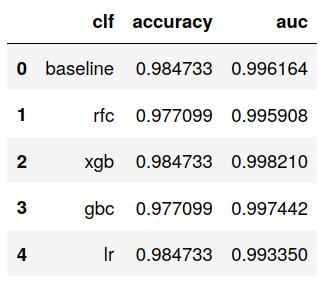
\includegraphics[width=5cm]{zdjecia/tabela.png}
\end{figure}

Sprawdziliśmy również jak skuteczne będą modele, jeśli usuniemy najbardziej skorelowana kolumnę z naszych danych. Okazuje się, że skuteczność modeli znacząco spada, bo aż o ok. 0.05.

\begin{figure}[!ht]
\centering
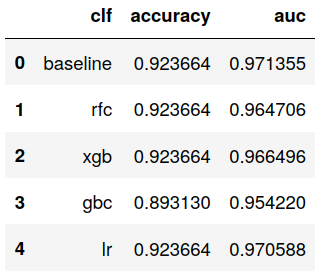
\includegraphics[width=5cm]{zdjecia/tabela_droped.png}
\end{figure}

\section{Podsumowanie}

Jesteśmy w stanie stworzyć model predykcyjny z ok. 98\% dokładnością. Najlepiej jest użyć XGBoost lub regresji logistycznej. 

\end{document}
